\subsubsection{从特征映射到核展开}
\label{sec:classic-overview-kernel-trick}

二分类模型在输入空间中划出一条边界：边界一侧预测正类，另一侧预测负类。原始坐标的加权和只能产生直线（二维时）或超平面（高维时）边界。若两类样本恰好能被一条直线分开，线性模型足够；但类别也可能按“到原点的距离是否小于 $1$”来区分，这时正类挤在单位圆内、负类散在圆外，任何一条直线都无法把整个圆内区域与圆外区域干净分开——无论直线画在哪里，圆的这一侧和那一侧都会同时出现两类点。

判断一个点在圆内还是圆外，需要的是半径平方 $x_1^2+x_2^2$。线性模型不认识平方项，但我们可以替它造出来：把 $x_1^2+x_2^2$ 整体当作一个新特征，再继续使用熟悉的线性得分。也就是说，不是让分类器在原坐标里硬画曲线，而是先把数据搬到一组新坐标，使在新坐标里分界重新变成直线。

图\ref{fig:classification-kernel-map}采用映射$\bm{\phi}(\bm{x})=(x_1,x_1^2+x_2^2)^{\top}$，将圆$x_1^2+x_2^2=1$对应到直线$\phi_2=1$。得分$g(\bm{x})=1-x_1^2-x_2^2$于是写成$g(\bm{x})=(0,-1)\bm{\phi}(\bm{x})+1$：对原坐标非线性，对新特征却是线性的。样本类别保持不变，改变的只是描述它们的坐标；图中边界是教学构造，并非由数据训练得到的最优分类边界。

\begin{figure}[htbp]
  \centering
  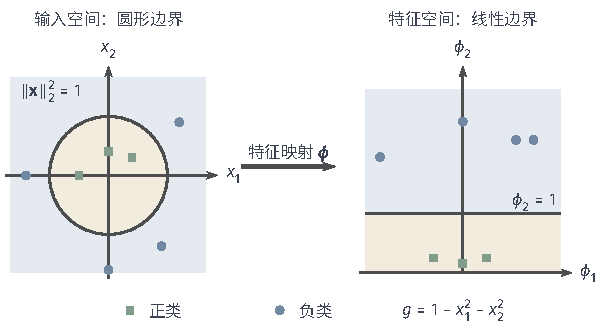
\includegraphics[width=103.166mm]{figures/04-classic-models/00-shared/tikz/classification-kernel-map/figure.pdf}
  \caption{非线性边界在特征映射前后的对应，两个面板的坐标均无量纲。正类方点为$(-0.5,0)$、$(0,0.4)$、$(0.4,0.3)$，负类圆点为$(-1.4,0)$、$(0,-1.6)$、$(1.2,0.9)$、$(0.9,-1.2)$。右图逐点使用$\phi_1=x_1$、$\phi_2=x_1^2+x_2^2$；水平线$\phi_2=1$对应左图半径为1的圆。数据与边界均为教学构造。}
  \label{fig:classification-kernel-map}
\end{figure}

圆形例子只需计算一个新特征，成本可以忽略。但若为了描述更复杂的弯曲关系而加入大量平方项、两两交互项甚至更高次项，显式列出所有新坐标就可能非常昂贵：仅二次映射，$d$ 个原变量就要产生约 $d^2/2$ 个新坐标，次数再升高数量还会快速增长；计算、存储和后续求解都要承担这份开销。于是出现一个关键问题：能不能在不真正写出、也不保存这些新坐标的情况下，照样完成计算？

\emph{从“只需内积”到核展开。}要回答这个问题，先检查线性算法到底怎样使用特征。给定$n$个训练输入$\bm x_1,\ldots,\bm x_n$，设$\bm\phi$将输入映射到带内积的特征空间$\mathcal H$，在那里使用线性得分$\langle\bm w,\bm\phi(\bm x)\rangle+b$。

在一类常见的训练问题里，训练损失只依赖各训练点的得分，而惩罚是参数范数的非减函数。把$\mathcal H$中的任意参数向量分解为“训练特征张成空间内的部分”与“正交于该空间的部分”：正交部分与每个训练特征的内积都是零，把它加到 $\bm w$ 上不会改变任何训练点的得分，却只会增大参数范数，从而增大惩罚。删去这一正交部分，训练得分不变、惩罚不增，因此若最优解存在，总能在这 $n$ 个训练特征张成的空间里找到它（张成空间＝这些特征向量线性组合能够到达的全部方向），即存在一组系数 $a_i$ 使
\begin{equation}
  \bm w=\sum_{i=1}^n a_i\bm\phi(\bm x_i).
  \label{eq:classic-overview-weight-expansion}
\end{equation}
这一展开只说明“有解时解可取在训练特征张成内”，并不单独证明解存在或唯一；存在性与唯一性仍由具体学习目标决定。

把这一展开代回线性得分，内积的线性性质允许把求和提到内积外面：
\begin{equation}
  \begin{aligned}
    K(\bm x,\bm z)
      &=\langle\bm\phi(\bm x),\bm\phi(\bm z)\rangle_{\mathcal H},\\
    f(\bm x)&=\sum_{i=1}^n a_iK(\bm x_i,\bm x)+b.
  \end{aligned}
  \label{eq:classic-overview-kernel}
\end{equation}
这里三者职责不同：核 $K$ 只给出两个输入映射后的特征内积，样本系数 $a_i$ 由具体学习目标确定，截距 $b$ 处理特征均值未被零化的整体偏移。预测时只需逐个计算新输入与训练输入的核值，既不必写出映射后的坐标，也不必保存高维的 $\bm w$。这种用核值完成特征内积计算的办法称为\term{核技巧}（kernel trick）；当$K$对原输入非线性时，特征空间中的线性得分也能描述原空间中的非线性关系，而显式特征展开这一步被完全绕过。

注意，式~\eqref{eq:classic-overview-kernel}只保证“预测”能改写为核值计算；要连训练也一起省去显式特征，训练问题本身也必须只通过核值使用特征。例如训练损失只使用各训练点的得分，并以正系数惩罚参数范数平方时，前面关于正交部分的论证正好适用：正交部分不改变训练得分却增加惩罚，最优解自然落在训练特征张成的空间内，于是整个训练都可用上述有限展开完成。具体到支持向量机，这一对偶形式将在分类章推导。核决定的是特征表示，分类、回归等任务仍由各自的损失和约束确定学习目标。

\subsubsection{合法核、常用核与超参数}
\label{sec:classic-overview-kernel-validity}
\label{sec:classic-overview-common-kernels}

\emph{什么样的函数才能充当核。}从“衡量相似性”的直觉随手设计一个 $K$ 并不困难，但不是每个看起来合理的相似性公式都能作为内积的替代。先注意这里说的“核”是特征内积的代称，与回归章局部加权里“按距离给记录加权重”的核只是同名：那个距离权重核只决定邻域内的加权平均，并不对应某个特征空间。原因在于，$K$ 必须真的等于某个特征空间中的内积，而内积有不能违反的代数性质。

内积首先是对称的：$\langle\bm u,\bm v\rangle=\langle\bm v,\bm u\rangle$。更重要的是，任意特征向量线性组合的长度平方都不可能为负。因此，对任意有限个输入$\bm x_1,\ldots,\bm x_m$和任意实系数$c_1,\ldots,c_m$，必须有
\[
  \begin{aligned}
    \sum_{i,j=1}^m c_ic_jK(\bm x_i,\bm x_j)
      &=\left\lVert\sum_{i=1}^m c_i\bm\phi(\bm x_i)\right\rVert^2\\
      &\geq0.
  \end{aligned}
\]
将这些输入的核值排成矩阵，称为这组输入的\term{Gram矩阵}（Gram matrix），也就是两两特征内积组成的矩阵；上述条件等价于矩阵对称且半正定，即用任意实向量 $\bm c$ 左乘右乘都不会得到负数。

反过来，若一个对称函数在整个预期输入域上对每一组有限输入都满足“Gram矩阵半正定”，就可以从形式特征的有限线性组合出发构造半内积（允许某个非零向量范数为零的退化内积），再把零范数的等价类消去、对空间完备化（补上所有极限点，使空间闭合），得到一个以该核为内积的特征空间。这里只交代存在性依据；连续性等Mercer定理的附加条件是针对特定定义域与连续核的进一步要求，不能误列为所有合法核的必要条件。本书将这样的函数称为正定核（positive definite kernel），允许有限核矩阵奇异（即存在非零 $\bm c$ 使二次型为零），不额外要求矩阵可逆。

合法性检查的是“所有实系数形成的二次型是否非负”，要避免几种常见误解。它不是检查每个核值本身是否非负——合法核在不相似的两点上完全可以取负值（例如未加常数的线性核）。它也不是凭“看起来像相似性”就能成立。只检查某一份训练集上的矩阵，只能确认这一组输入合法；新输入还必须落在核已确认合法的定义域内。此外，合法核只提供“它确实对应某个特征内积”的依据，并不保证这个特征表示适合当前任务，也不保证对应的学习目标容易求解——合法性与有效性是两件事。

对$\bm x,\bm z\in\mathbb R^d$，选择不同的核，等于暗中选择了不同的特征空间和特征关系。表\ref{tab:classic-overview-common-kernels}列出常见形式及条件；核尺度记为$\beta$，多项式次数记为$p$，与输入维数$d$区分。

\begin{table}[htbp]
  \centering
  \small
  \begin{tabularx}{\linewidth}{@{}>{\RaggedRight\arraybackslash}p{18mm}>{\RaggedRight\arraybackslash}X>{\RaggedRight\arraybackslash}p{27mm}@{}}
    \toprule
    名称 & $K(\bm{x},\bm{z})$ & 参数与正定性\\
    \midrule
    线性核 & $\bm{x}^{\top}\bm{z}$ & 半正定\\
    多项式核 & $(\beta\bm{x}^{\top}\bm{z}+r)^p$ & $\beta,r\ge0$，正整数$p$\\
    高斯RBF核 & $\exp(-\beta\lVert\bm{x}-\bm{z}\rVert_2^2)$ & $\beta>0$，半正定\\
    Laplacian核 & $\exp(-\beta\lVert\bm{x}-\bm{z}\rVert_1)$ & $\beta>0$，半正定\\
    Sigmoid形式 & $\tanh(\beta\bm{x}^{\top}\bm{z}+r)$ & 一般不保证半正定\\
    \bottomrule
  \end{tabularx}
  \caption{常用核函数与合法性条件。这里的“半正定”要求任意有限输入的Gram矩阵半正定；Sigmoid一行列出的是常见相似性形式，使用前仍需针对定义域与参数核验。}
  \label{tab:classic-overview-common-kernels}
\end{table}

\term{线性核}（linear kernel）就是原始特征的内积，不增加任何新特征，对应普通的线性模型，常作为比较基准。\term{多项式核}（polynomial kernel）隐式加入了有限阶的特征交互：把 $(\beta\bm x^\top\bm z+r)^p$ 展开后，各项对应原变量的各次乘积，因此 $p=2$ 时能表达平方项和两两乘积，$p$ 更大时表达更高次的组合。在$\beta>0$时，$r=0$只保留$p$次项，$r>0$则包含从常数项到$p$次项的各阶特征；参数取零时，相应特征块可以消失。核计算省去的是这些坐标的显式展开，完整训练成本仍取决于样本数和学习目标。

\term{高斯径向基核}（Gaussian radial basis function kernel，Gaussian RBF kernel）不看方向上的投影，而按两点的欧氏距离衡量局部接近程度：两点重合时核值为 $1$，距离越远核值平滑衰减到 $0$。常将$\beta$写成$1/(2\sigma^2)$，其中$\sigma>0$是距离尺度：$\sigma$ 越大（$\beta$ 越小），核值衰减越慢，一个点能影响的范围越宽；$\sigma$ 越小（$\beta$ 越大），作用范围越局部。它对应的特征空间是无限维的，因而能表达相当灵活的非线性关系，但作用范围是否合适仍需结合数据判断，不能仅凭“能拟合弯曲边界”就断定新样本误差更小。

\term{Laplacian核}（Laplacian kernel）形式相近，只是把欧氏距离换成$L^1$距离，即各坐标绝对差之和；$L^1$距离沿坐标轴方向变化，改变了衡量“接近”的几何，对某些坐标轴对齐的结构更敏感。

常称为\term{Sigmoid核}（sigmoid kernel）的形式把内积送入双曲正切函数，在神经网络兴起后常被使用，但它一般不保证正定核所需的半正定性；只取正参数也不足以替代对定义域和参数取值的合法性核验，使用前必须单独检查或改用其他核。核尺度、多项式次数、正则化强度等在一次拟合前固定的配置，可以用验证数据在训练内选择；配置确定后，还要用未参与选择的新数据评价预测误差，不能把选择配置时用过的数据再当作最终评价依据。

\subsubsection{核矩阵与训练中心}
\label{sec:classic-overview-kernel-matrix}

把预测公式用于全部训练点，可以看出核方法的规模压力落在哪里。训练时，将$n$个输入两两之间的核值排成训练Gram矩阵$\bm K\in\mathbb R^{n\times n}$，其中$\bm K_{i,j}=K(\bm x_i,\bm x_j)$。令$\bm a=(a_1,\ldots,a_n)^{\top}$、$\bm1\in\mathbb R^n$为全一向量，式\eqref{eq:classic-overview-kernel}在训练点上的预测便是$\bm K\bm a+b\bm1$。完整存储这个矩阵需要$O(n^2)$空间，构造它需要$O(n^2)$次核计算；也就是说，核技巧把“显式展开可能极高维的特征”的压力，转换成了“成对计算并存储样本关系”的压力，后续求解线性或二次问题的成本还要另外计算。当样本量很大时，这一 $n^2$ 规模往往比特征维数更先成为瓶颈，省去显式坐标并不等于没有计算代价。

有些学习目标要求比较样本围绕共同中心的变化，而不是它们相对原点的绝对位置。例如核PCA要在特征空间中找“数据散布最大的方向”，这一分析应当围绕特征均值进行；原点位置改变不应影响结论。这时需要在特征空间中减去训练均值。训练特征均值与各点的偏离量为
\[
  \bar{\bm\phi}=\frac1n\sum_{i=1}^n\bm\phi(\bm x_i),
  \qquad
  \widetilde{\bm\phi}_i=\bm\phi(\bm x_i)-\bar{\bm\phi}.
\]
中心化后的内积仍可只用核值计算。令$\bm I_n$为单位矩阵，中心化矩阵和中心化核矩阵为
\begin{equation}
  \bm H=\bm I_n-\frac1n\bm1\bm1^{\top},
  \qquad \bm K_{\mathrm c}=\bm H\bm K\bm H.
  \label{eq:classic-overview-kernel-centering}
\end{equation}
矩阵 $\bm H$ 的作用就是“减去平均值”：左乘或右乘 $\bm H$ 相当于减去行均值或列均值。有限维特征按行排成矩阵$\bm\Phi$时，减去每列训练均值得到$\bm H\bm\Phi$，其Gram矩阵就是$\bm H\bm\Phi\bm\Phi^{\top}\bm H=\bm H\bm K\bm H$。即使特征空间是无限维的，无法写出矩阵 $\bm\Phi$，直接展开中心化特征的内积也得到同一个公式 $\bm H\bm K\bm H$，这正是核技巧的价值所在。还要注意，非线性映射与减均值一般不能交换次序，因此只在原输入空间做中心化，并不能代替在特征空间中的这一步。

新输入$\bm x$在预测时也必须减去同一个训练特征均值，保持训练和预测使用共同参照；不能为每个新查询重新定义中心，否则训练得到的坐标与预测坐标不在同一参照系中。它与第$i$个训练输入的中心化核值为
\[
  \begin{aligned}
    K_{\mathrm c}(\bm x_i,\bm x)
      ={}&K(\bm x_i,\bm x)
       -\frac1n\sum_{j=1}^n K(\bm x_i,\bm x_j)\\
       &-\frac1n\sum_{j=1}^n K(\bm x_j,\bm x)
       +\frac1{n^2}\sum_{j,l=1}^n K(\bm x_j,\bm x_l).
  \end{aligned}
\]
四项可以逐项对照 $\langle\bm\phi(\bm x_i)-\bar{\bm\phi},\bm\phi(\bm x)-\bar{\bm\phi}\rangle$ 的展开来理解：第一项是原内积，第二、三项分别扣除两个端点与训练均值的内积，最后一项把均值自身的内积加回来，因为它在前两步里被减了两次。所有求和都固定使用训练输入，新点不参与均值的计算。是否中心化由学习目标决定：核PCA这类分析围绕特征均值变化的方法需要中心化，而直接做分类、回归的核方法未必需要；采用核并不意味着所有方法都执行同一套中心化流程。
